% !TEX root = ../main.tex

\section{Simulation of seesaw perceptron}

The seesaw perceptron with variable input size was created using the Visual DSD syntax through an abstraction layer written in Javascript. The software can take the truth table that should be fulfilled as an array. A seesaw perceptron with the correct number of input gates and the correct left and right recognition sequences is then automatically generated. For example, using the software with the 2-input AND gate (\tref{and_table}) would generate the sequences seen in \fref{seesaw_neuron}. The source code is available on Github \cite{neuralcompiler}.

To train the perceptron, a row from the truth table is run through the Visual DSD simulation. Looking at the first row from \tref{and_table}, the Visual DSD code for a 2-input perceptron is generated, with input 1 and input 2 concentrations of 0 nM, a weight of 0 and threshold of 10 (see \fref{seesaw_neuron_schematic}). A time analysis is then done in Visual DSD of the output strand concentration. If the output concentration is equal to the output from the first row of the truth table (within a margin of error), the result is accepted, and the simulation moves on to the next row of the truth table. For the next row, new Visual DSD code is generated with input 1 concentration of 0 nM, and input 2 concentration of 1 nM. The output concentration is analyzed again. If the output is not equal to the one defined in the truth table, the weights of the perceptron is increased by 0.1, and the simulation is run for the next row of the truth table. This is repeated until a weight is found, where all rows from the truth table produces the correct output when run through the seesaw perceptron. This is summarized in \lref{codetraining}.

To test the perceptron compiling and training, 5 different truth tables were used, ranging from 2 to 3 inputs (\cref{2_and,2_or,3_and,3_1_or,3_2_or}). The correct output was reached after 16-23 iterations of the learning algorithm. Input sizes greater than 3 were not tested, as the training time increases exponentially in time with the input size. Only truth tables that didn't involve NOT and XOR logic were used, as no solutions exist to these problems with the current algorithm (no linear separability and negative weights).


\subsection{2-input AND}

\begin{figure}[H]
  \begin{subfigure}[t]{.49\columnwidth}

      \centering
    \begin{tabular}[b]{ccc}
      \hline
      \multicolumn{1}{l}{\textbf{Input 1}} & \multicolumn{1}{l}{\textbf{Input 2}} & \multicolumn{1}{l}{\textbf{Output}} \\
      \hline
      0                                    & 0                                    & 0                                   \\
      0                                    & 1                                    & 0                                   \\
      1                                    & 0                                    & 0                                   \\
      1                                    & 1                                    & 1 \\
      \hline
    \end{tabular}
    \caption{Truth table for the 2-input AND gate.}
  \end{subfigure}
  \begin{subfigure}[t]{.49\textwidth}
    \includegraphics[width=\textwidth]{figures/trained_2_and.tikz}
    \caption{Diagram of the 2-input AND with correct weights and threshold.}
  \end{subfigure}
\hfill
\begin{subfigure}[t]{\textwidth}
  \centering
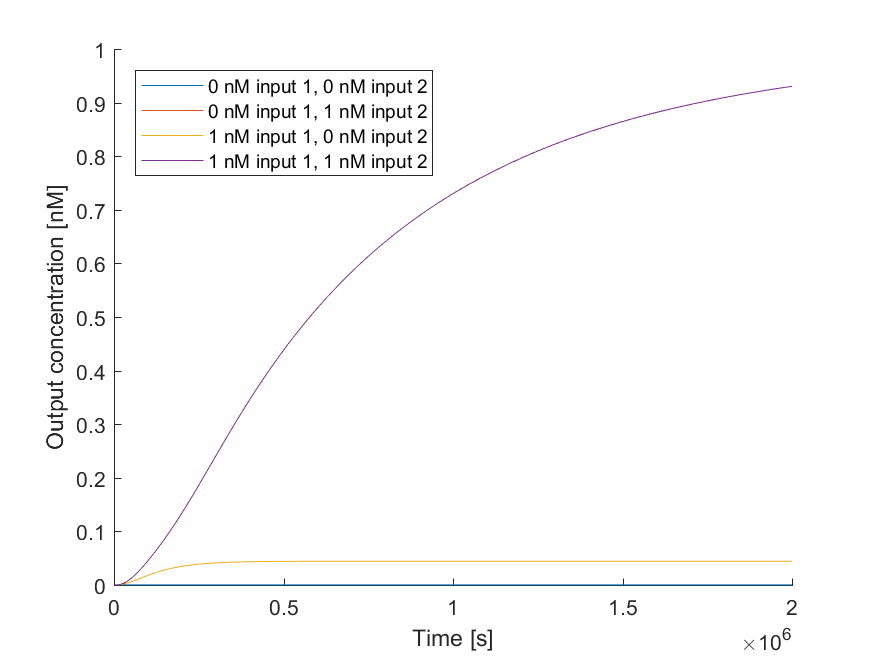
\includegraphics[width=\textwidth]{images/and_simulation.png}
\caption{Time analysis of the 2-input AND.}
\end{subfigure}
\caption{Simulation results of the trained 2-input AND gate. The network is trained to activate when both of the inputs are active. The correct output was obtained after 21 iterations of the training algorithm, with a weight of 1.9 for all inputs, and a threshold of 10.}
\label{2_and}
\end{figure}

\subsection{2-input OR}

\begin{figure}[H]
  \begin{subfigure}[t]{.49\columnwidth}

      \centering
    \begin{tabular}[b]{ccc}
      \hline
    \multicolumn{1}{l}{\textbf{Input 1}} & \multicolumn{1}{l}{\textbf{Input 2}} & \multicolumn{1}{l}{\textbf{Output}} \\
    \hline
    0                                    & 0                                    & 0                                   \\
    0                                    & 1                                    & 1                                   \\
    1                                    & 0                                    & 1                                   \\
    1                                    & 1                                    & 1 \\
    \hline
    \end{tabular}
    \caption{Truth table for the 2-input OR gate.}
\end{subfigure}
\begin{subfigure}[t]{.49\textwidth}
  \includegraphics[width=\textwidth]{figures/trained_2_or.tikz}
  \caption{Diagram of the 2-input OR with correct weights and threshold.}
\end{subfigure}
\hfill
\begin{subfigure}[t]{\textwidth}
  \centering
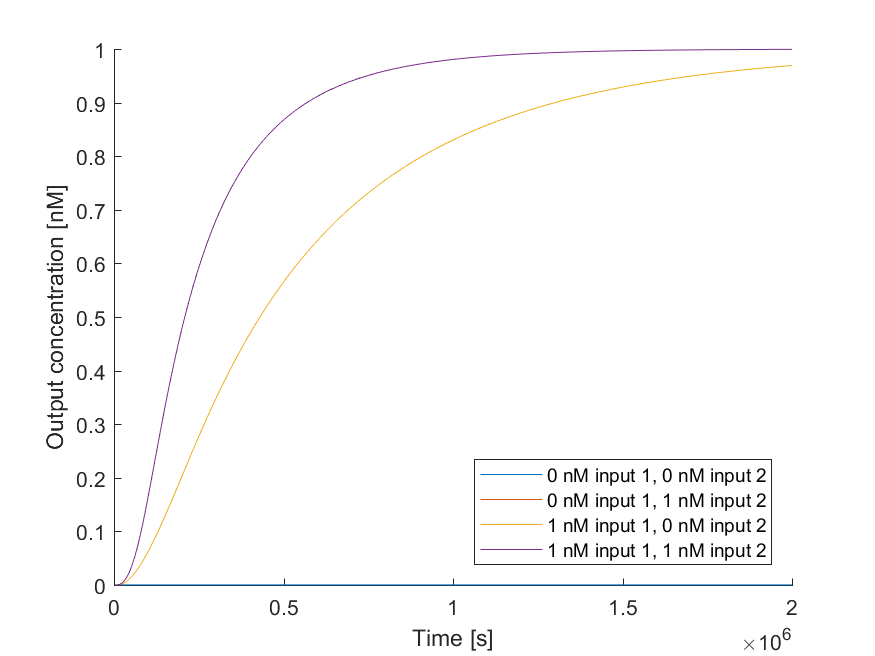
\includegraphics[width=\textwidth]{images/or_simulation.png}
\caption{Time analysis of the 2-input OR.}
\end{subfigure}
\caption{Simulation results of the trained 2-input OR gate. The network is trained to activate when one of the inputs is active. The correct output was obtained after 22 iterations of the training algorithm, with a weight of 2.1 for all inputs, and a threshold of 10.}
\label{2_or}
\end{figure}

\subsection{3-input AND}

\begin{figure}[H]
  \begin{subfigure}[t]{.49\columnwidth}
    \begin{adjustbox}{width=\textwidth}
    \begin{tabular}[b]{cccc}
      \hline
    \multicolumn{1}{l}{\textbf{Input 1}} & \multicolumn{1}{l}{\textbf{Input 2}} & \multicolumn{1}{l}{\textbf{Input 3}} & \multicolumn{1}{l}{\textbf{Output}} \\
    \hline
    0 & 0                                    & 0                                    & 0                                   \\
    0 & 0                                    & 1                                    & 0                                   \\
    0 & 1                                    & 0                                    & 0                                   \\
    0 & 1                                    & 1                                    & 0                                   \\
    1 & 0                                    & 0                                    & 0                                   \\
    1 & 0                                    & 1                                    & 0                                   \\
    1 & 1                                    & 0                                    & 0                                   \\
    1 & 1                                    & 1                                    & 1                                   \\

    \hline
    \end{tabular}
  \end{adjustbox}
    \caption{Truth table for the 3-input AND gate.}
\end{subfigure}
\begin{subfigure}[t]{.49\textwidth}
  \includegraphics[width=\textwidth]{figures/trained_3_and.tikz}
  \caption{Diagram of the 3-input AND with correct weights and threshold.}
\end{subfigure}
\hfill
\begin{subfigure}[t]{\textwidth}
  \centering
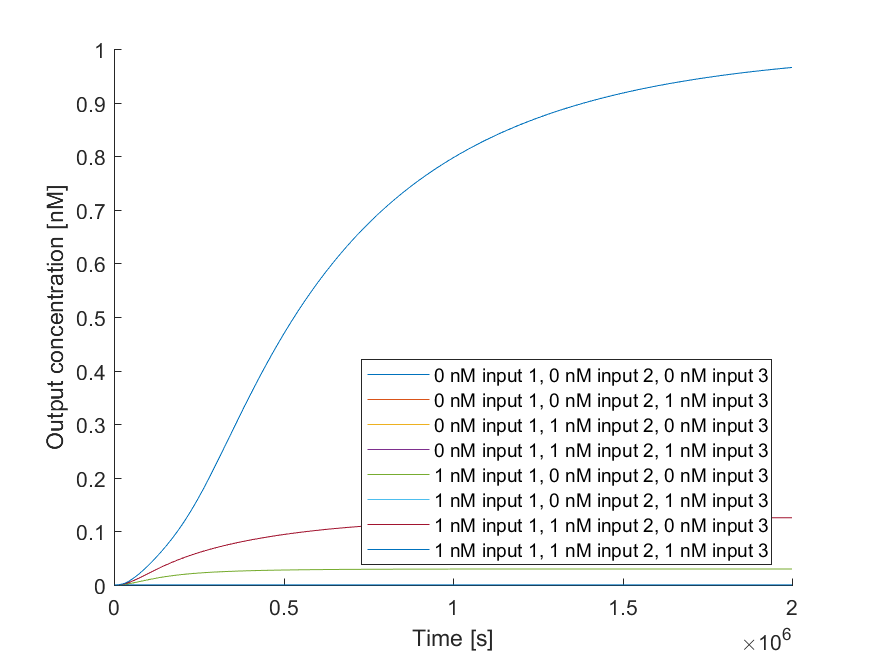
\includegraphics[width=\textwidth]{images/and_simulation_3input.png}
\caption{Time analysis of the 3-input AND.}
\end{subfigure}
\caption{Simulation results of the trained 3-input AND gate. The network is trained to activate when all of the inputs are active. The correct output was obtained after 14 iterations of the training algorithm, with a weight of 1.2 for all inputs, and a threshold of 10.}
\label{3_and}
\end{figure}

\subsection{3-input 1-OR}

\begin{figure}[H]
  \begin{subfigure}[t]{.49\columnwidth}

      \begin{adjustbox}{width=\textwidth}
    \begin{tabular}[b]{cccc}
      \hline
    \multicolumn{1}{l}{\textbf{Input 1}} & \multicolumn{1}{l}{\textbf{Input 2}} & \multicolumn{1}{l}{\textbf{Input 3}} & \multicolumn{1}{l}{\textbf{Output}} \\
    \hline
    0 & 0                                    & 0                                    & 0                                   \\
    0 & 0                                    & 1                                    & 1                                   \\
    0 & 1                                    & 0                                    & 1                                   \\
    0 & 1                                    & 1                                    & 1                                   \\
    1 & 0                                    & 0                                    & 1                                   \\
    1 & 0                                    & 1                                    & 1                                   \\
    1 & 1                                    & 0                                    & 1                                   \\
    1 & 1                                    & 1                                    & 1                                   \\

    \hline
    \end{tabular}
  \end{adjustbox}
    \caption{Truth table for the 3-input 1-OR gate.}
\end{subfigure}
\begin{subfigure}[t]{.49\textwidth}
  \includegraphics[width=\textwidth]{figures/trained_3_1_or.tikz}
  \caption{Diagram of the 3-input 1-OR with correct weights and threshold.}
\end{subfigure}
\hfill
\begin{subfigure}[t]{\textwidth}
  \centering
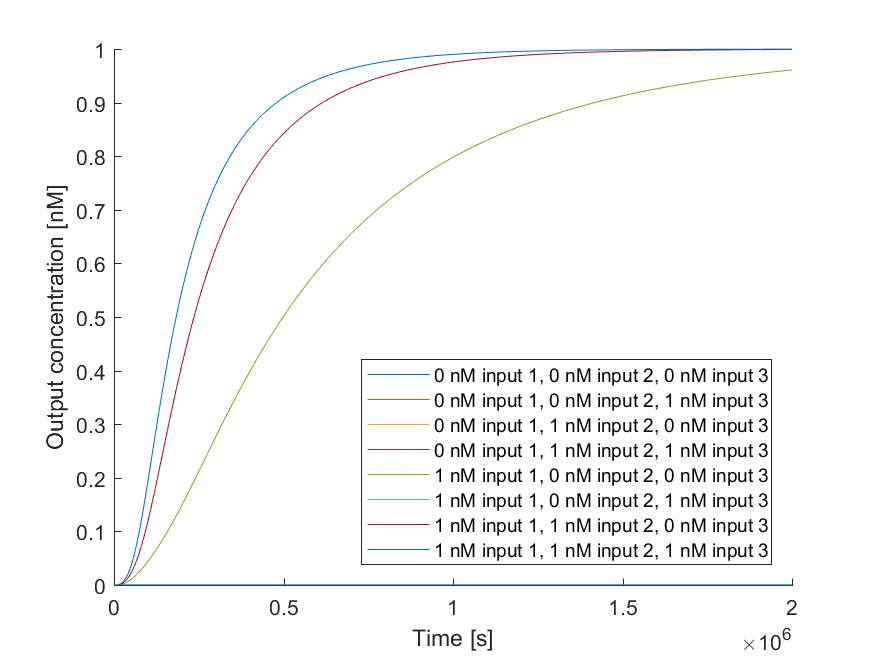
\includegraphics[width=\textwidth]{images/or_1_simulation_3input.png}
\caption{Time analysis of the 3-input 1-OR.}
\end{subfigure}
\caption{Simulation results of the trained 3-input 1-OR gate. The network is trained to activate when at least 1 of the inputs is active. The correct output was obtained after 16 iterations of the training algorithm, with a weight of 1.3 for all inputs, and a threshold of 10.}
\label{3_1_or}
\end{figure}

\subsection{3-input 2-OR}


\begin{figure}[H]
  \begin{subfigure}[t]{.49\columnwidth}
    \begin{adjustbox}{width=\textwidth}
    \begin{tabular}[b]{cccc}
      \hline
    \multicolumn{1}{l}{\textbf{Input 1}} & \multicolumn{1}{l}{\textbf{Input 2}} & \multicolumn{1}{l}{\textbf{Input 3}} & \multicolumn{1}{l}{\textbf{Output}} \\
    \hline
    0 & 0                                    & 0                                    & 0                                   \\
    0 & 0                                    & 1                                    & 0                                   \\
    0 & 1                                    & 0                                    & 0                                   \\
    0 & 1                                    & 1                                    & 1                                   \\
    1 & 0                                    & 0                                    & 0                                   \\
    1 & 0                                    & 1                                    & 1                                   \\
    1 & 1                                    & 0                                    & 1                                   \\
    1 & 1                                    & 1                                    & 1                                   \\

    \hline
    \end{tabular}
  \end{adjustbox}
    \caption{Truth table for the 3-input 2-OR gate.}
\end{subfigure}
\begin{subfigure}[t]{.49\textwidth}
  \includegraphics[width=\textwidth]{figures/trained_3_2_or.tikz}
  \caption{Diagram of the 3-input 2-OR with correct weights and threshold.}
\end{subfigure}
\hfill
\begin{subfigure}[t]{\textwidth}
  \centering
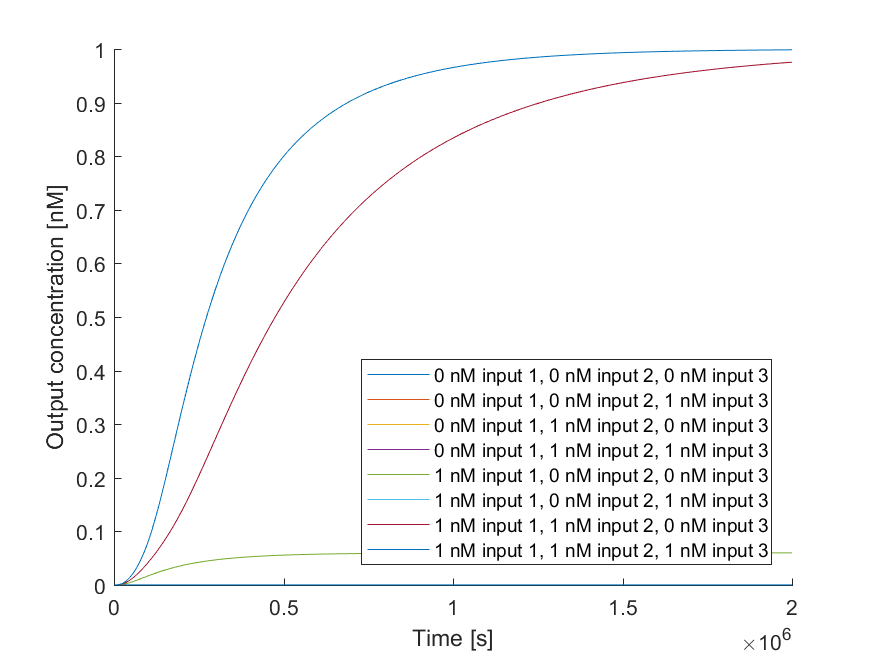
\includegraphics[width=\textwidth]{images/or_2_simulation_3input.png}
\caption{Time analysis of the 3-input 2-OR.}
\end{subfigure}
\caption{Simulation results of the trained 3-input 2-OR gate. The network is trained to activate when at least 2 of the inputs is active. The correct output was obtained after 15 iterations of the training algorithm, with a weight of 1.4 for all inputs, and a threshold of 10.}
\label{3_2_or}
\end{figure}

\section{Translation of RNA sequences}

\subsection{Translator design}

The sequences for the RNA translator was designed to output CUAGACUGAAGCUCCUUGAGG, through two strand displacement reactions. The design was done in Nupack using the code in \lref{codeshort} for the short translator and \lref{codelong} for the long translator. The resulting RNA sequences from Nupack can be seen in \tref{rna_strands}. The RNA was converted to the required DNA template for transcription using a custom program \cite{nupackorder}, which implements the process shown in \fref{rna_to_dna_process}. The template DNA strands required for the transcription can be seen in \tref{dna_strands}. Refer to \fref{translator_short_subunits,translator_long_subunits} for the naming of the strands.

\begin{table}
\begin{adjustbox}{width=\columnwidth}
\begin{tabular}{llll}
\hline
\textbf{Name}      & \textbf{Short} & \textbf{Sequence}                                           & \textbf{Length} \\
\hline
T7 promoter        & 0          & GGTAATACGACTCACTATAG                                           & 20     \\
Short 1            & 1          & CCTCAAGGAGCTTCAGTCTAGCCCTATAGTGAGTCGTATTACC                    & 43     \\
Short 2            & 2          & CTCCTTGAGGCACATAACTCCCCTATAGTGAGTCGTATTACC                     & 42     \\
Short 3            & 3          & CACATAACTCTACTAAATCTCCCTATAGTGAGTCGTATTACC                     & 42     \\
Short 4            & 4          & GAGTTATGTGCCTCAAGGAGCCCTATAGTGAGTCGTATTACC                    & 42     \\
Short 5            & 5          & AGATTTAGTAGAGTTATGTGCCCTATAGTGAGTCGTATTACC                     & 42     \\
Long 1             & 6          & GTCAATTCGCCTCAAGGAGCTTCAGTCTAGCCCTATAGTGAGTCGTATTACC           & 52     \\
Long 2             & 7          & GCTCCTTGAGGCGAATTGACCCATCTTCATTCTACTCCTACCCTATAGTGAGTCGTATTACC & 62     \\
Long 3             & 8          & CCATCTTCATTCTACTCCTATACCTCAATCCCCTATAGTGAGTCGTATTACC           & 52     \\
Long 4             & 9          & TAGGAGTAGAATGAAGATGGGTCAATTCGCCTCAAGGAGCCCCTATAGTGAGTCGTATTACC & 62     \\
Long 5             & 10         & GATTGAGGTATAGGAGTAGAATGAAGATGGCCCTATAGTGAGTCGTATTACC           & 52     \\
Beacon fluorophore & 11         & CGGCTAGACTGAA                                                  & 13     \\
Beacon quencher    & 12         & CCTCAAGGAGCTTCAGTCTAGCCG                                       & 24 \\
\hline
\end{tabular}
\end{adjustbox}
\caption{Sequences and names of the DNA strands used for transcription.}
\label{dna_strands}
\end{table}

\begin{table}
\begin{adjustbox}{width=\columnwidth}
\begin{tabular}{llll}
\hline
\textbf{Name}      & \textbf{Short} & \textbf{Sequence}                                           & \textbf{Length} \\
\hline
Short 1            & 1          & GGCUAGACUGAAGCUCCUUGAGG                    & 23     \\
Short 2            & 2          & GGGAGUUAUGUGCCUCAAGGAG                     & 22     \\
Short 3            & 3          & GGAGAUUUAGUAGAGUUAUGUG                     & 22     \\
Short 4            & 4          & GGCUCCUUGAGGCACAUAACUC                     & 22     \\
Short 5            & 5          & GGCACAUAACUCUACUAAAUCU                     & 22     \\
Long 1             & 6          & GGCUAGACUGAAGCUCCUUGAGGCGAAUUGAC           & 32     \\
Long 2             & 7          & GGUAGGAGUAGAAUGAAGAUGGGUCAAUUCGCCUCAAGGAGC & 42     \\
Long 3             & 8          & GGGAUUGAGGUAUAGGAGUAGAAUGAAGAUGG           & 32     \\
Long 4             & 9          & GGGCUCCUUGAGGCGAAUUGACCCAUCUUCAUUCUACUCCUA & 42     \\
Long 5             & 10         & GGCCAUCUUCAUUCUACUCCUAUACCUCAAUC           & 32     \\
% Beacon fluorophore & 11         & CGGCTAGACTGAA                                                  & 13     \\
% Beacon quencher    & 12         & CCTCAAGGAGCTTCAGTCTAGCCG                                       & 24 \\
\hline
\end{tabular}
\end{adjustbox}
\caption{Sequences and names of the transcribed RNA strands.}
\label{rna_strands}
\end{table}

% The gels from the transcription, annealing, and PCR reactions is shown here. As it was not possible to get the correct RNA sequences needed for fluorescence measurements, there are no strand displacement results to compare with the results from the original article \cite{Picuri2009}.

\subsection{Transcription}

The result of the DNA template annealing can be seen in \fref{promoter_annealing_gel}. The darkest bands are the annealed samples. The samples for the short translator runs at about the same size, while there is bigger variation in the long translator samples, as expected based on \tref{dna_strands}. The exact positions of the long translator samples does not match with the sequence length, though this can be explained by secondary structures of the single-stranded part of the sample. The shorter bands visible below, are probably excess promoter, other secondary structures, and shorter sequences from synthesis errors. No lane with ladder was run, so the exact position of the bands can't be commented on.


\begin{figure}[h]
\begin{subfigure}[t]{0.54\textwidth}
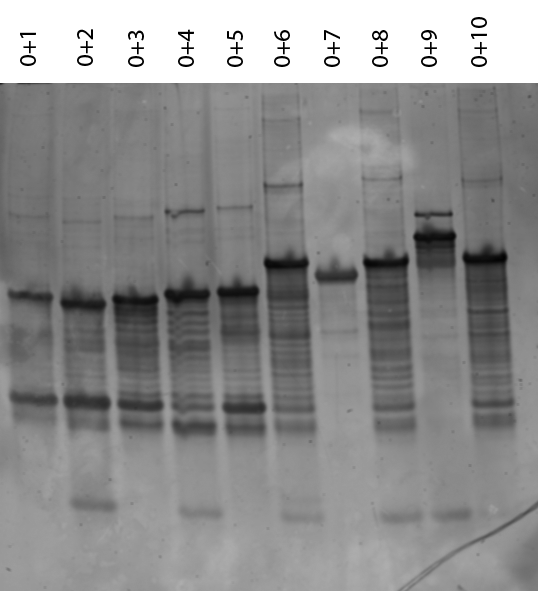
\includegraphics[width=\textwidth]{images/promoter_annealing_gel.png}
\caption{}
\label{promoter_annealing_gel}
\end{subfigure}
\begin{subfigure}[t]{0.46\textwidth}
  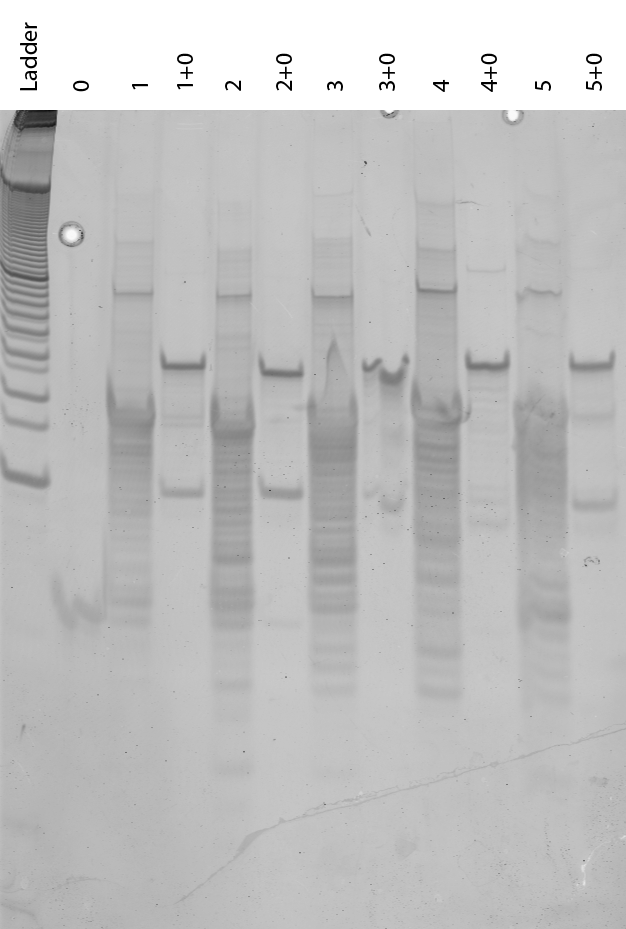
\includegraphics[width=\textwidth]{images/translator_annealing_2.png}
  \caption{}
  \label{translator_annealing_2}
\end{subfigure}
\caption{\subref{promoter_annealing_gel} Typhoon scan of the annealed templates and promoter strands. The lanes are labelled by which strands are annealed (see table \ref{dna_strands}). \subref{translator_annealing_2} The annealed strands again, together with the single strands as controls and a 10 nt ladder. The lanes are labelled with the strand names given in \tref{dna_strands}. The plus symbol denotes which strands are annealed.}
\end{figure}

The transcription result of the annealed templates can be seen in \fref{transcriptions}. The lanes 1-10 does not show distinct bands. There seems to be more product from the long translator transcriptions (lanes 6-10), than in the short ones (lanes 1-5). Even the controls (lanes 11 and 12) which were loaded in equal amounts does not show up in equal strength. Since the gel from the DNA annealing was run without any controls, it was difficult to see if there was any errors in the annealing. To simplify the experiment while trying to find the error, only the short translator sequences were used, and a new annealing gel with proper controls was run (\fref{translator_annealing_2}).

\begin{figure}[h]
  \begin{subfigure}[t]{0.49\textwidth}
  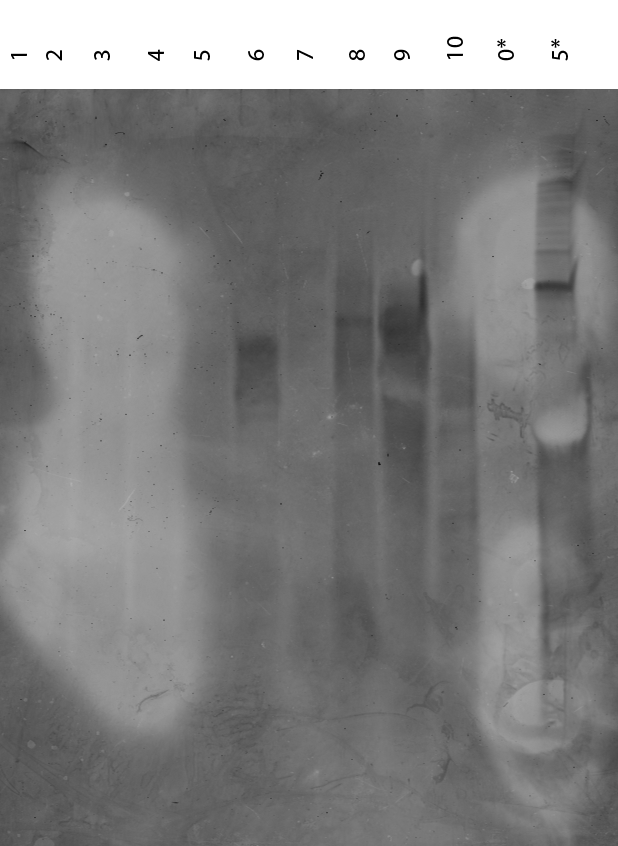
\includegraphics[width=\textwidth]{images/translator_transcription_1.png}
  \caption{}
  \label{transcription_1}
  \end{subfigure}
  \begin{subfigure}[t]{0.49\textwidth}
    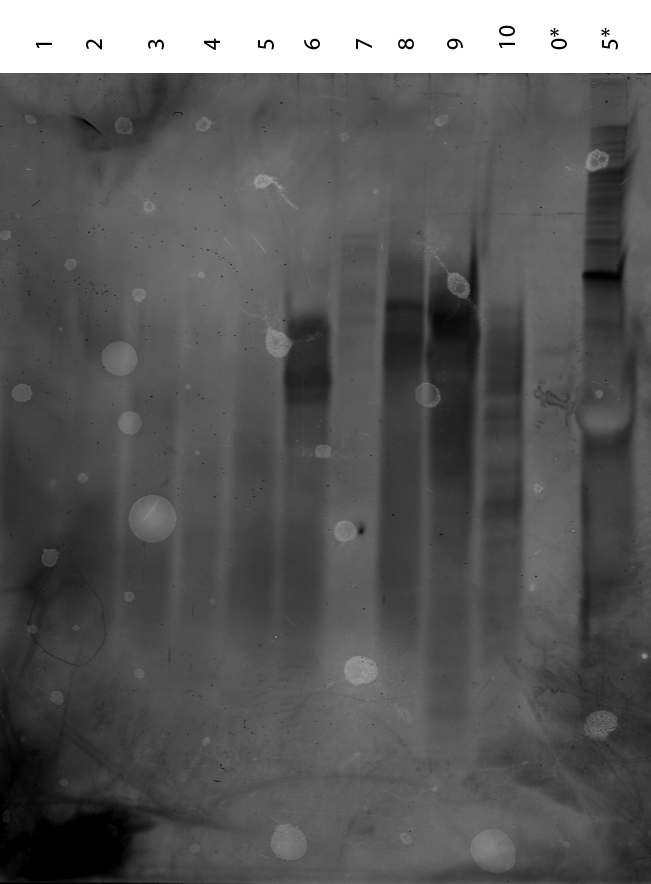
\includegraphics[width=\textwidth]{images/translator_transcription_2.png}
    \caption{}
    \label{transcription_2}
  \end{subfigure}
  \caption{\subref{transcription_1} Typhoon scan of the transcribed RNA strands in lanes 1-10, and the original DNA strands as controls in 11 and 12. The lanes are labelled by which strands are annealed (see \tref{rna_strands}). The asterix refers to the DNA strands in \tref{dna_strands}. \subref{transcription_2} The same gel after further staining in SYBR Gold.}
  \label{transcriptions}
\end{figure}


The results of \fref{translator_annealing_2} still shows that the templates have annealed with the promoter, and runs as about 40-50 bp. The expected size is around 60 bp if the template was fully double-stranded (sum of promoter and template), but it is difficult to say how a partly annealed structure will run on a native gel. The new gel does however show that the bands in the annealed lanes below the assumed product, might not be excess promoter. The promoter is seen in the second lane, and lies below the bands in the annealed structure thought to be excess promoter. The bands below the product might be due to secondary structures of each of the template strands, but comparing with \fref{short_secondary_structures}, the band in the 5+0 lane would be expected to be less visible, as strand 5 has no secondary structure.

Despite the unexplained bands from the annealing, a new transcription was run on the short template strands to see if better results could be obtained. The UV shadowing still did not show any visible product, so the gel was scanned to check for bands (\fref{translator_transcription_3}).

\begin{figure}[h]
\begin{subfigure}[t]{.43\textwidth}
  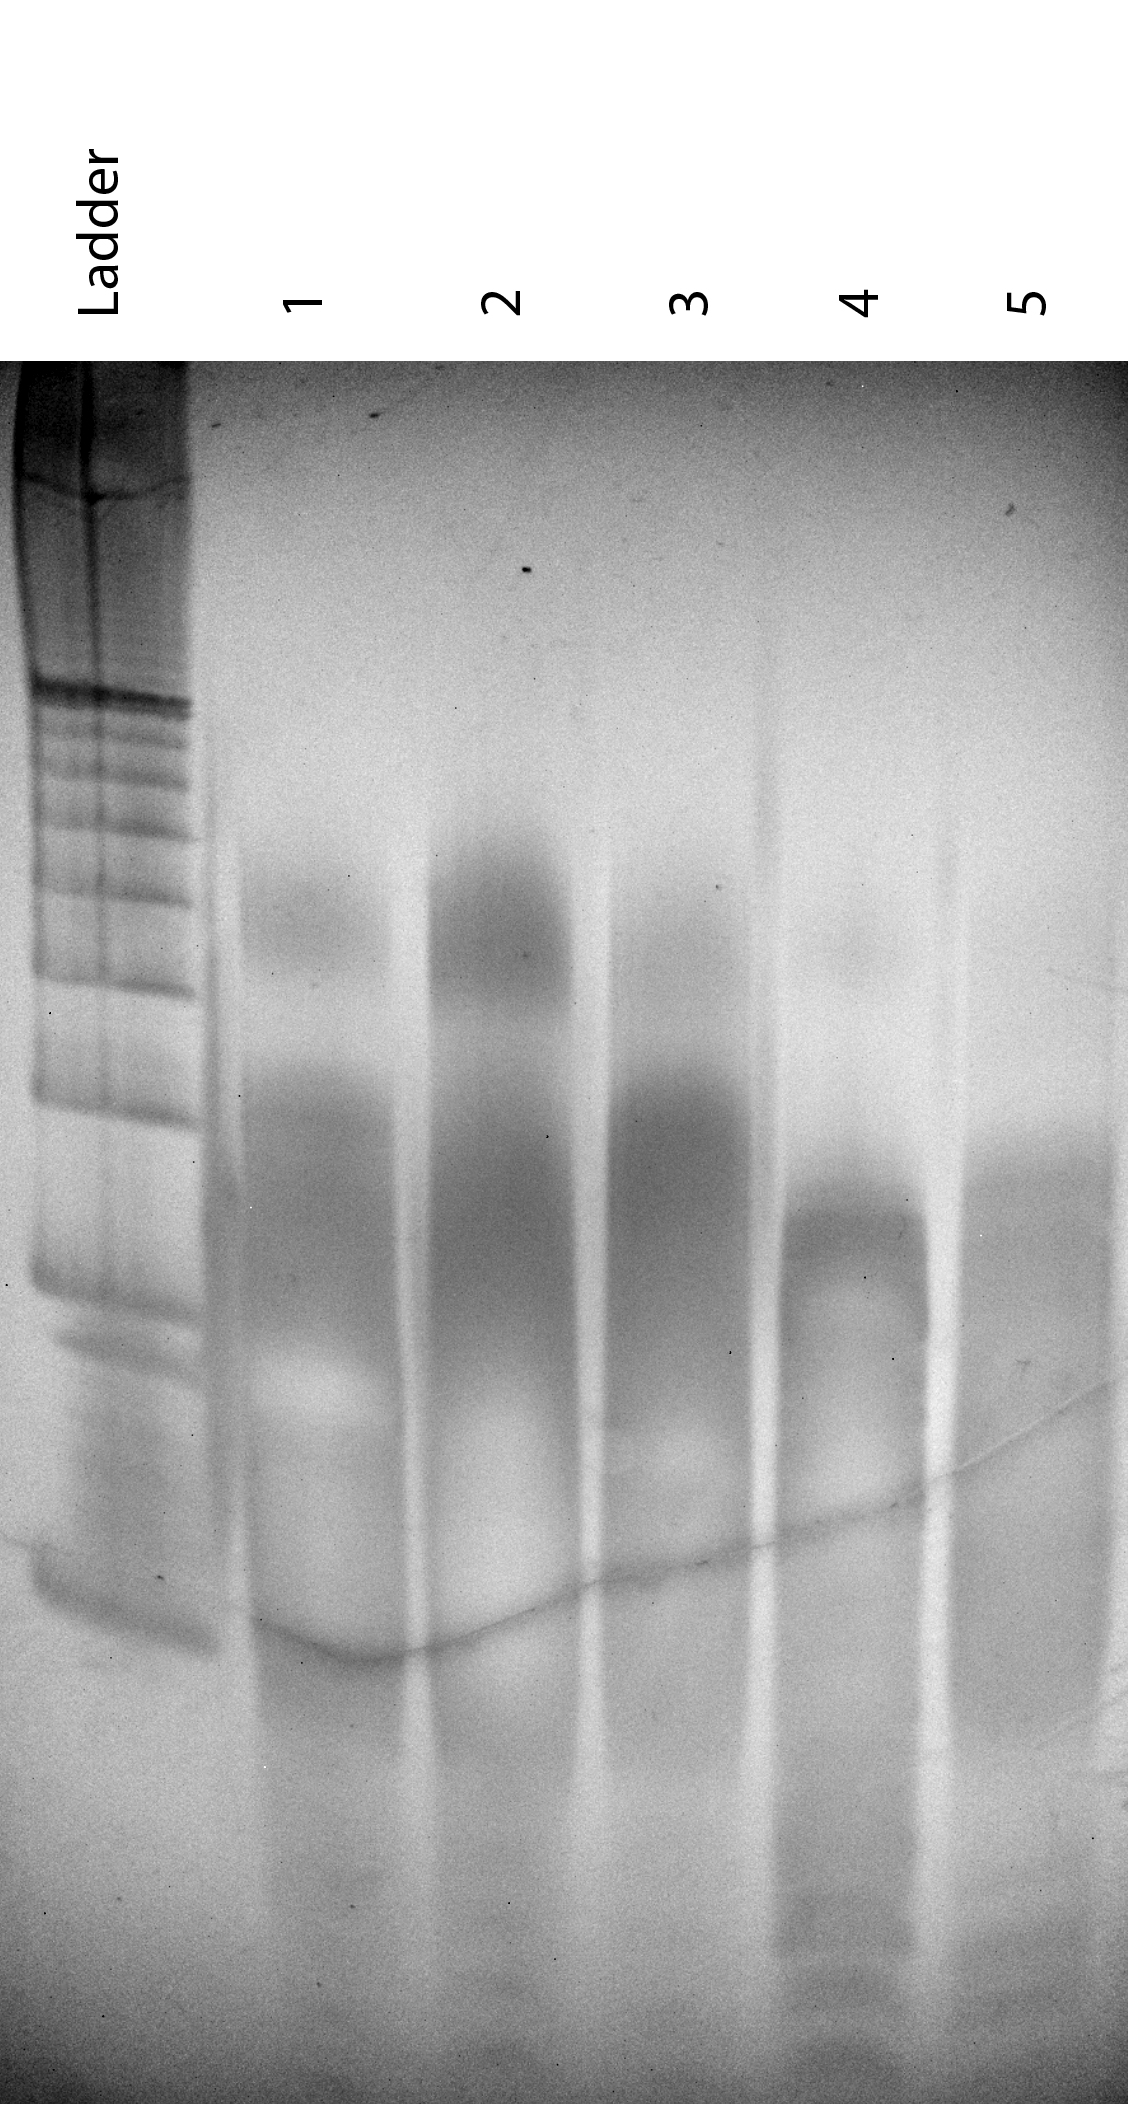
\includegraphics[width=\textwidth]{images/translator_transcription_3.png}
  \caption{}
  \label{translator_transcription_3}
\end{subfigure}
\begin{subfigure}[t]{.55\textwidth}
  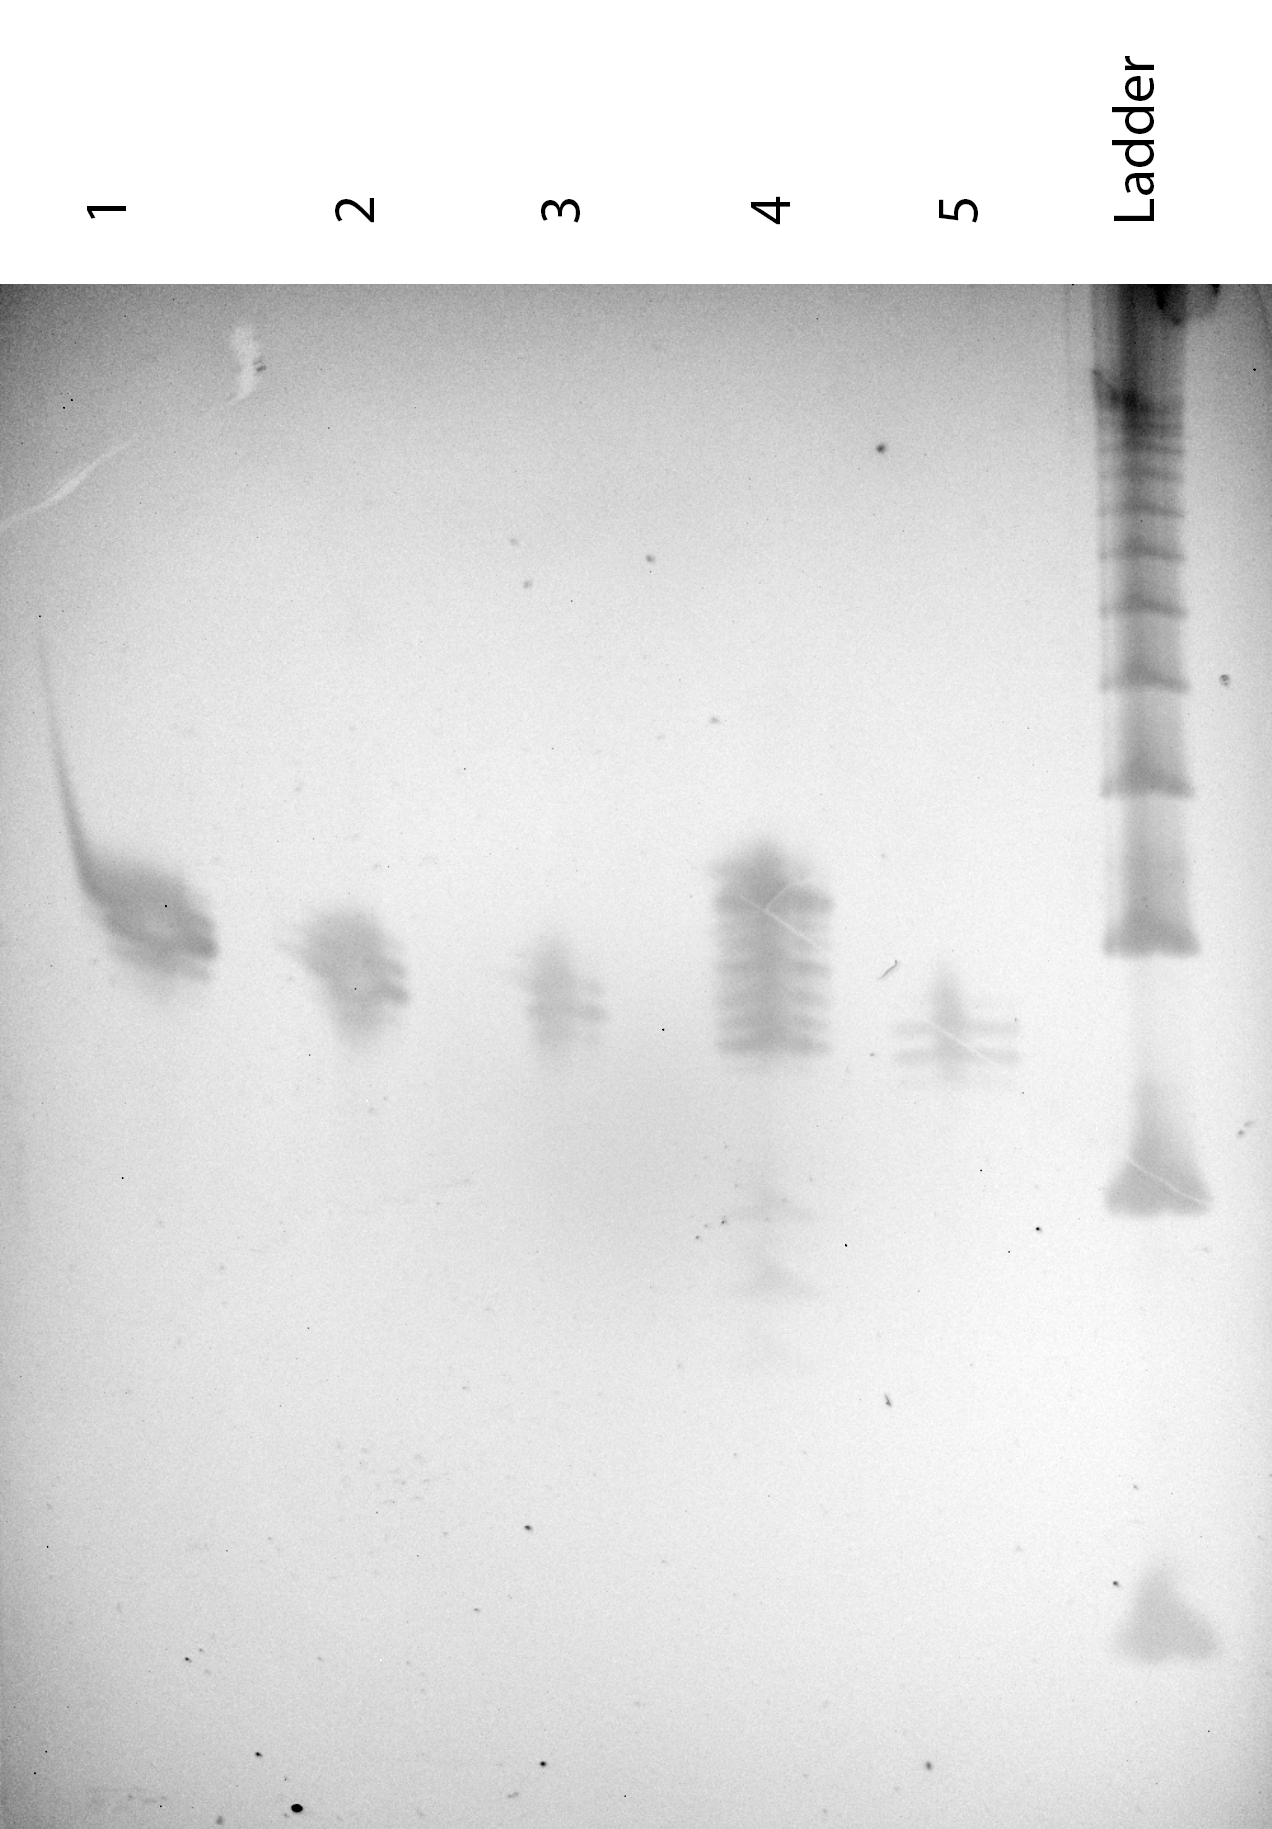
\includegraphics[width=\textwidth]{images/translator_transcription_purified.png}
  \caption{}
  \label{translator_transcription_purified}
\end{subfigure}
\caption{\subref{translator_transcription_3} The transcribed short translator sequences and a 10 nt ladder. The lanes are labelled with the strand names given in \tref{rna_strands}. \subref{translator_transcription_purified} The purified short translator RNA strands with a 10 nt ladder.}
\end{figure}

As seen in \fref{translator_transcription_3}, still no clear bands with RNA product was visible. After checking all buffers and materials, it was learned that the T7 polymerase that was used was from 2013, and might have been too old to still function properly. A fresh T7 polymerase was used for a new transcription. The UV shadowing did show some distinct bands this time, so the bands were cut out for purification.

\fref{translator_transcription_purified} shows that the RNA has been isolated, but is not very pure. It is possible that when cutting out the RNA from the gel before purification, too large an area was taken. The target RNA sequences were still expected to be in the purified samples (albeit not very pure), and it has previously been shown that strand displacement reactions can work with unpurified components \cite{Thubagere2017}, so the experiment continued with the current RNA.

The result of the annealed RNA translators and the reporter can be seen in \fref{transcription_annealed}. It was expected that the fluorophore would be visible at the same wavelength as SYBR Gold, so a scan without staining should show the free fluorophore (and not the quenched fluorophore in the annealed reporter).

\begin{figure}[h]
\begin{subfigure}[t]{.5\textwidth}
  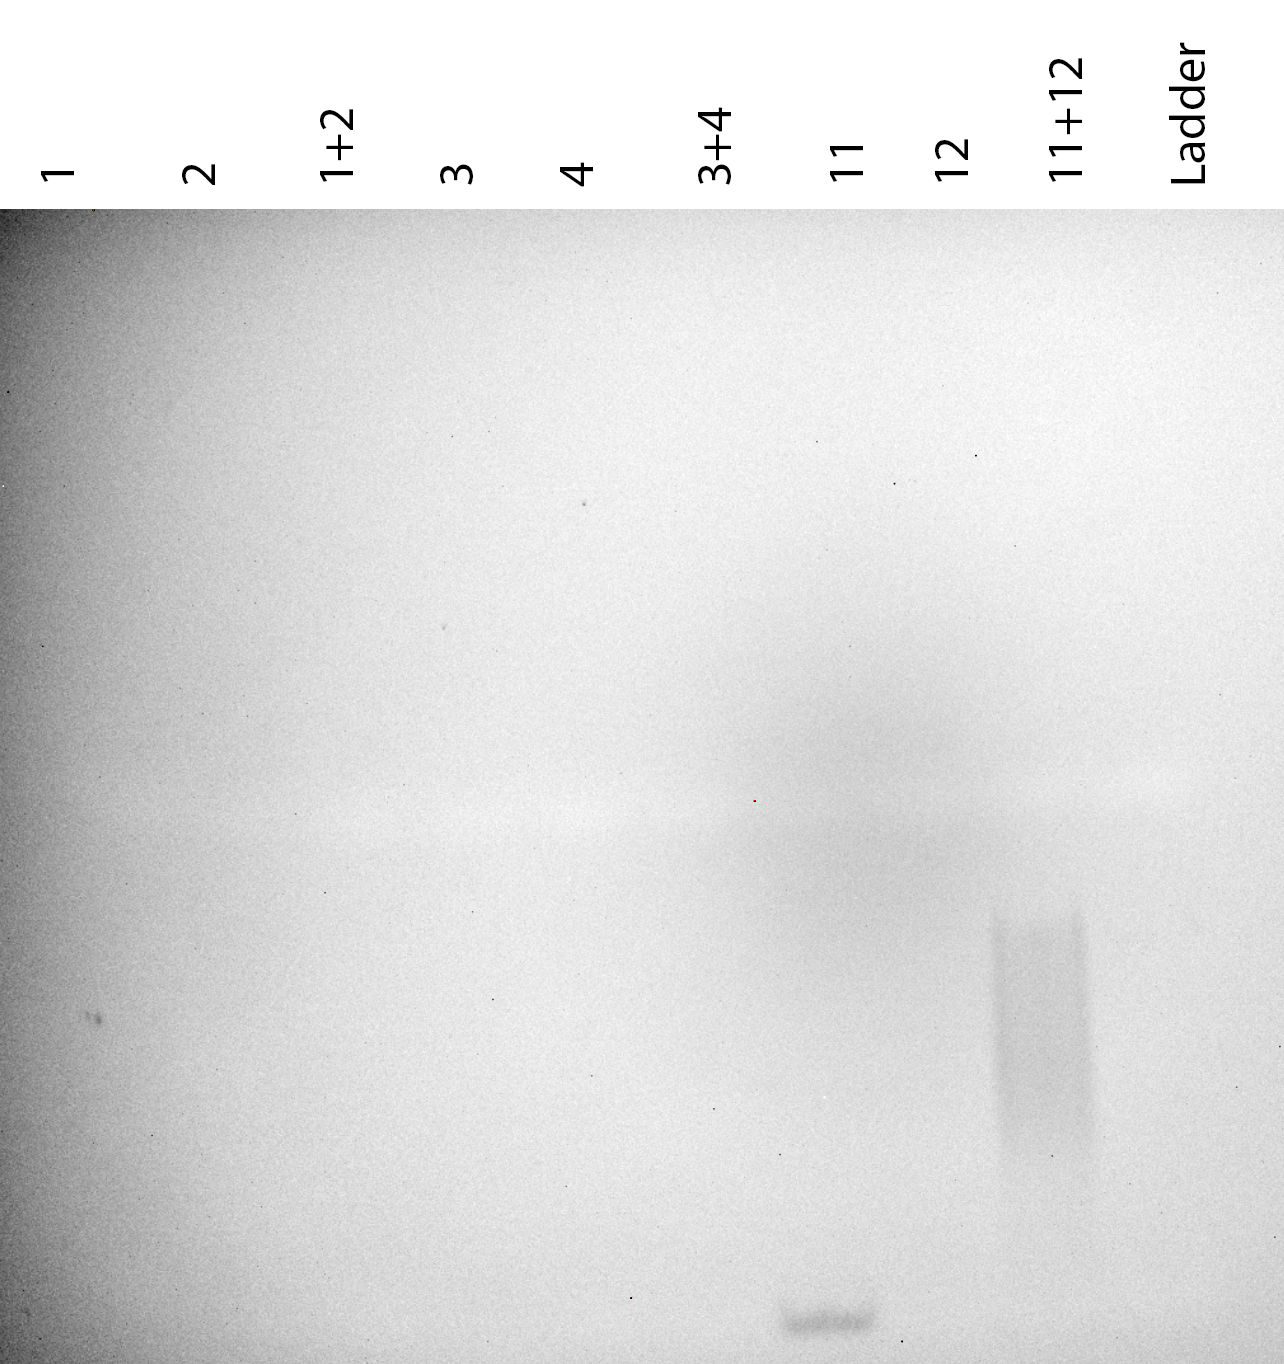
\includegraphics[width=\textwidth]{images/transcription_annealed_nostain.png}
  \caption{Not stained}
  \label{transcription_annealed_nostain}
\end{subfigure}
\begin{subfigure}[t]{.5\textwidth}
  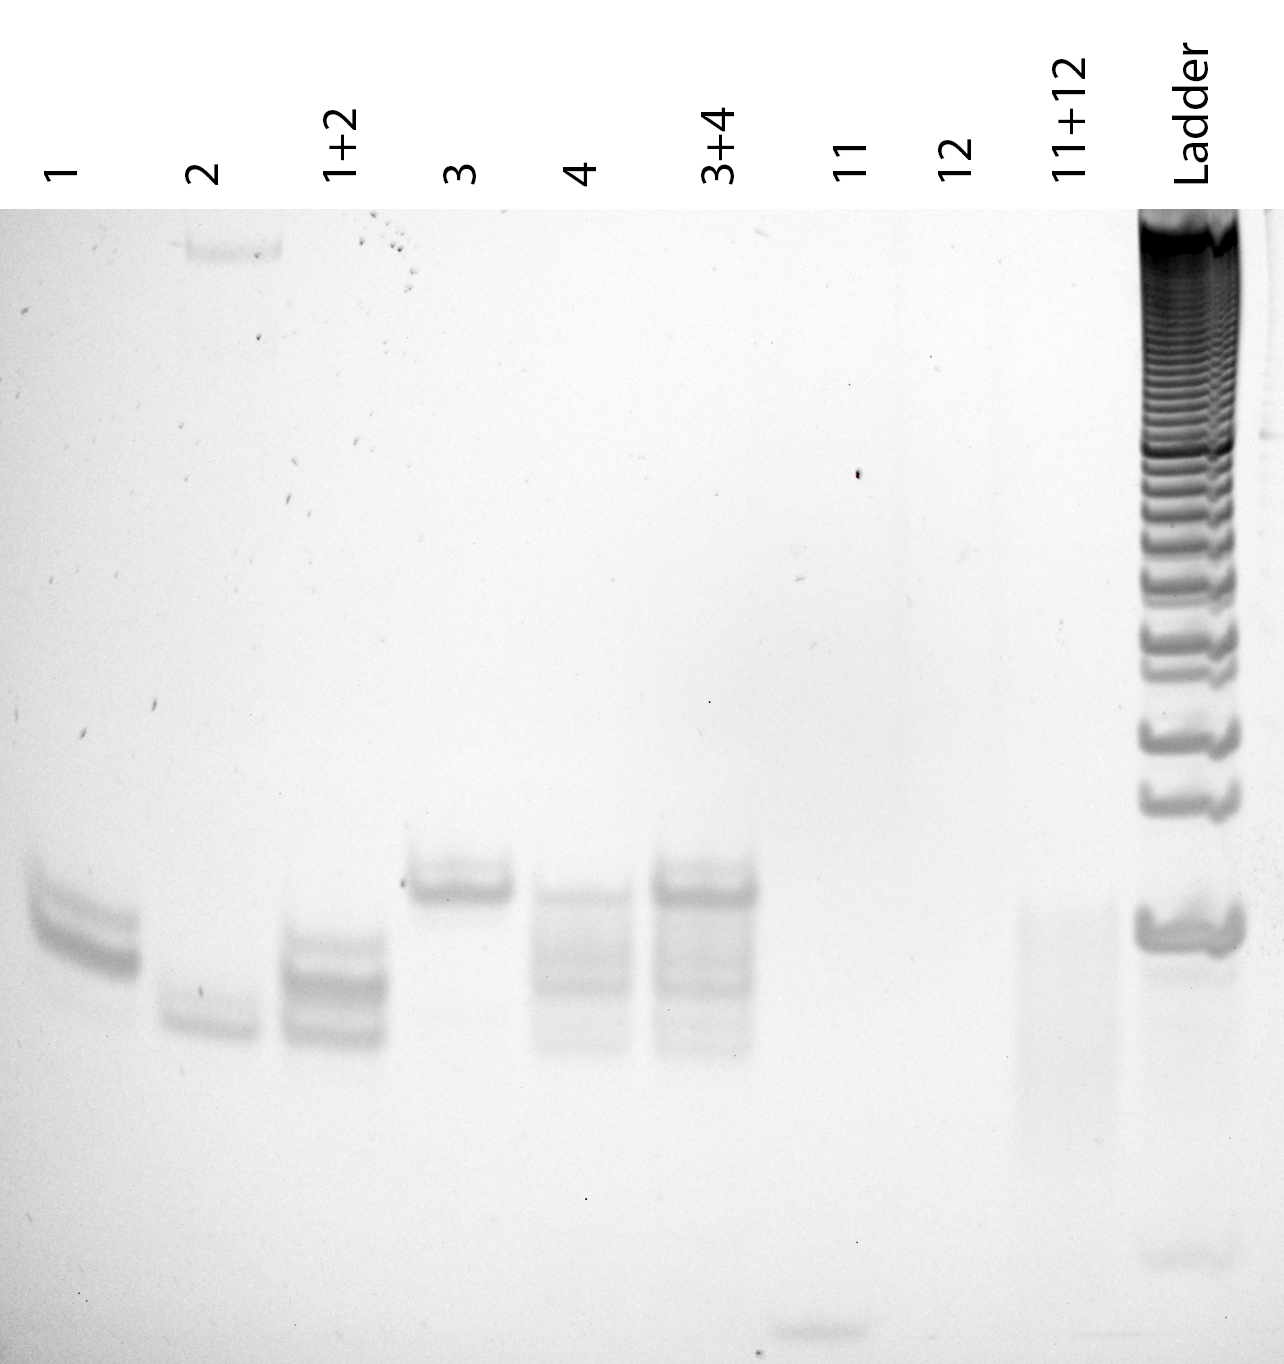
\includegraphics[width=\textwidth]{images/transcription_annealed_stain.png}
  \caption{Stained}
  \label{transcription_annealed_stain}
\end{subfigure}
\caption{The annealed short translator subunits and reporter, with the single strands as controls, and a 10 nt ladder.}
\label{transcription_annealed}
\end{figure}

As seen in \fref{transcription_annealed_nostain}, the fluorophore clearly shows up in the unstained scan, and gets partly quenched and moves up when annealed to its quencher. The smear in the annealed reporter might be due to synthesis errors in the quencher strand.

In the stained scan (\fref{transcription_annealed_stain}), the annealed half-translators does not seem to have annealed at all. Comparing with the controls, the strands that were supposed to have annealed, merely looks like the sum of the single strands. There is a few reasons why this could have happened. The RNA that was purified from gel was not the correct sequences, the annealing was not carried out correctly, or the strands simply doesn't anneal very well.

To check the strength of the annealing, the strands were analyzed in Nupack. The free energy analysis (\fref{annealing_concentration}) shows that the short translator sequences does not anneal as well as the long ones. Due to time constraints, the focus moved towards the long translator sequences, as they were expected to provide better results.

The long translator sequences were transcribed using the first transcription protocol. The result can be seen in \fref{translator_transcription_long_1}.

\begin{figure}[h]
\begin{subfigure}[t]{0.51\textwidth}
  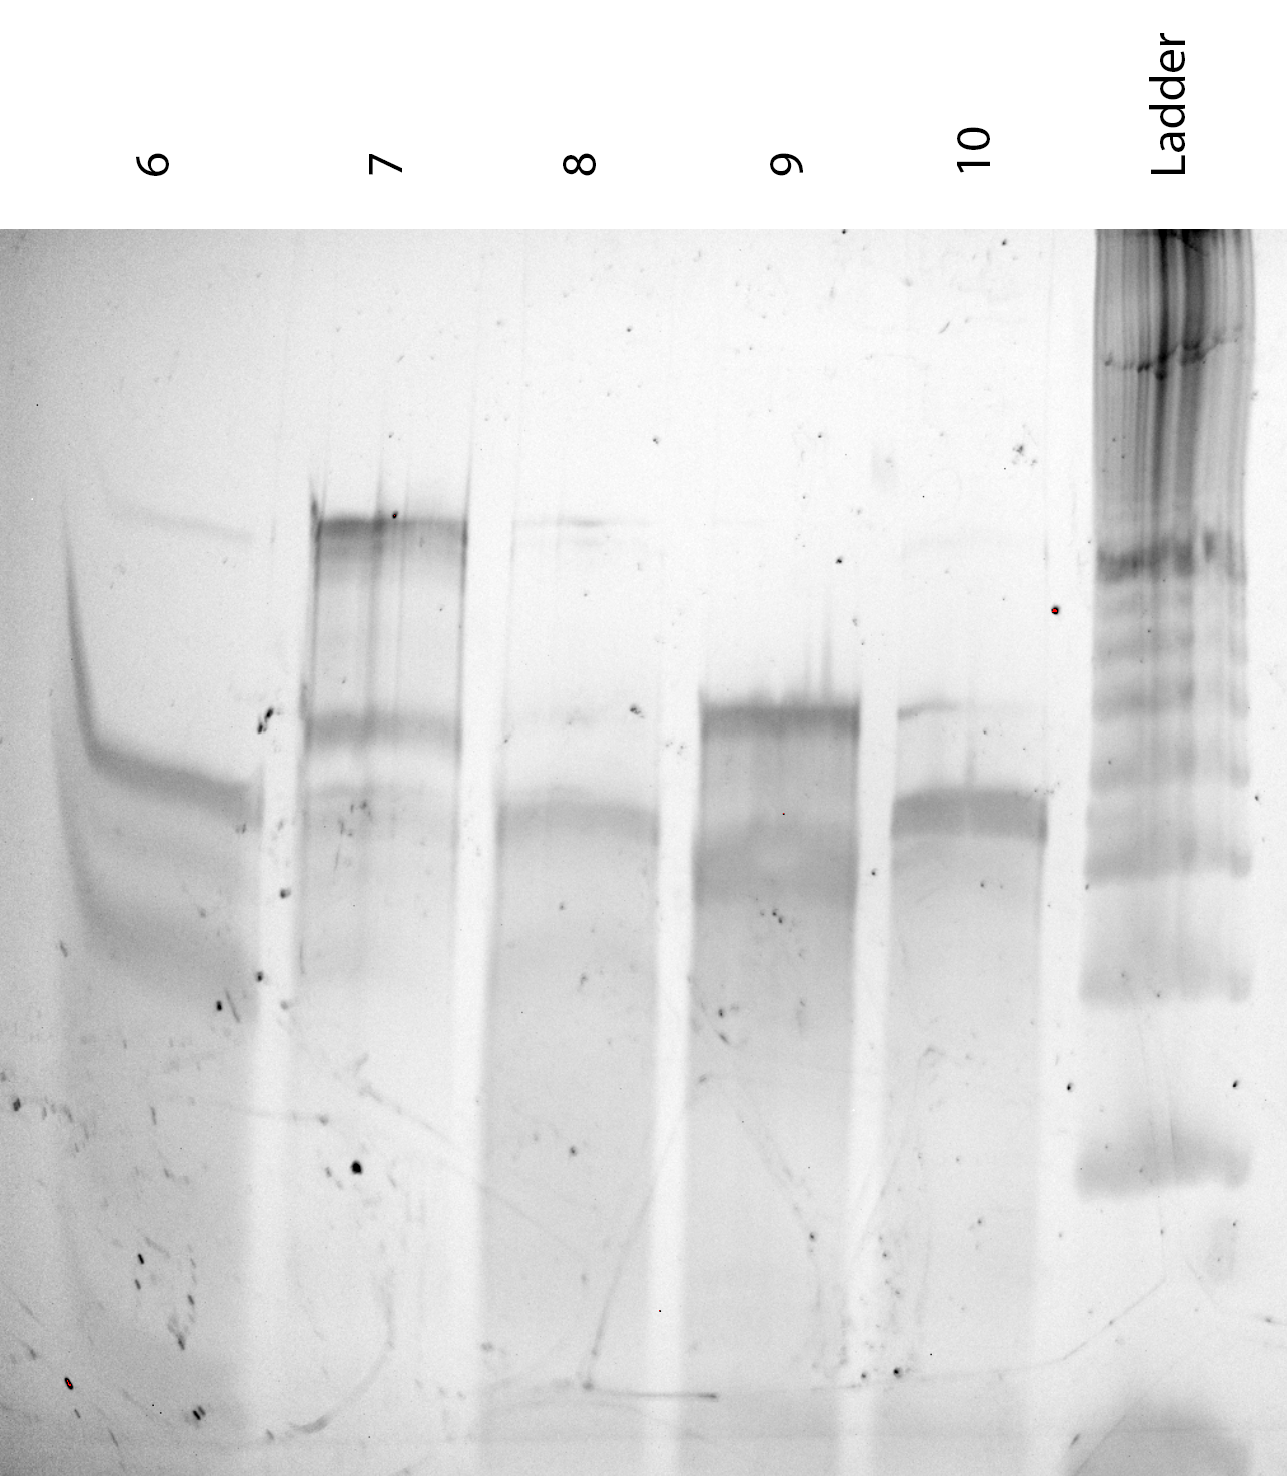
\includegraphics[width=\textwidth]{images/translator_transcription_long_1.png}
  \caption{}
  \label{translator_transcription_long_1}
\end{subfigure}
\begin{subfigure}[t]{0.49\textwidth}
  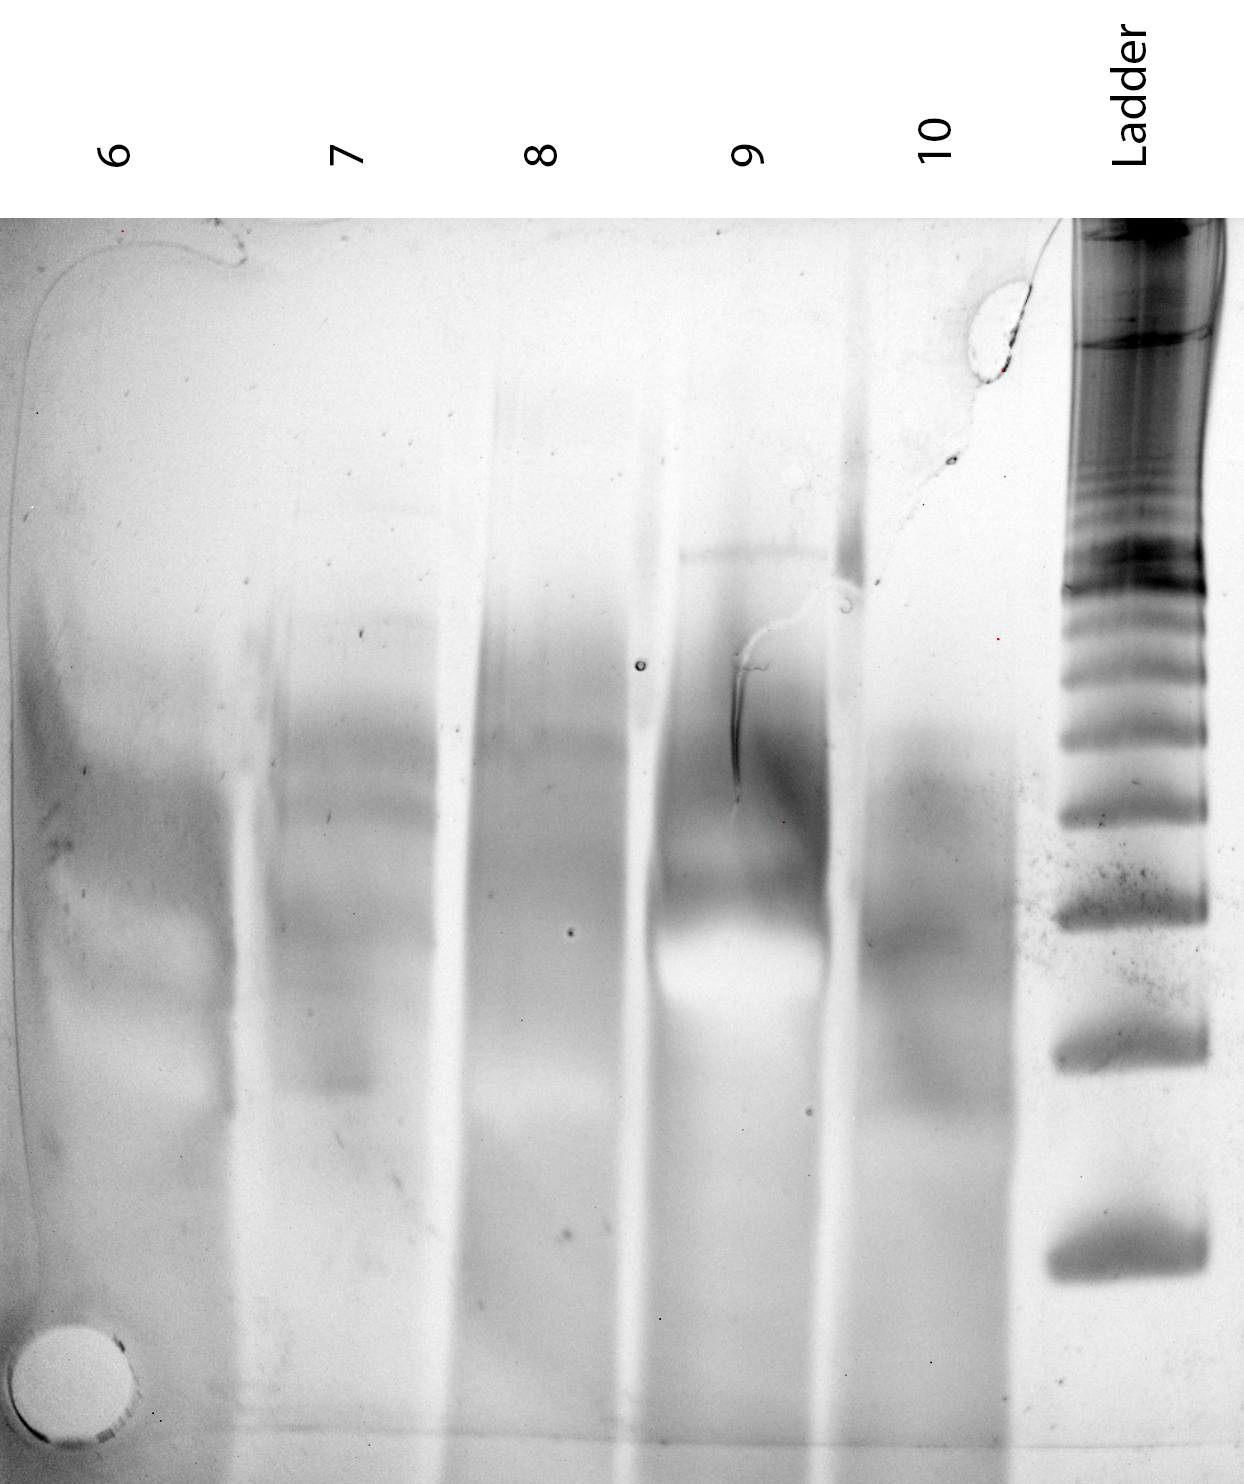
\includegraphics[width=\textwidth]{images/translator_transcription_long_2.png}
  \caption{}
  \label{translator_transcription_long_2}
\end{subfigure}
\caption{\subref{translator_transcription_long_1} Transcription of the long translator sequences with a 10 nt ladder. \subref{translator_transcription_long_2} Transcription of the long translator sequences with a 10 nt ladder, using an adapted protocol.}
\end{figure}

As seen in \fref{translator_transcription_long_1}, some RNA was produced so the concentration of nucleotides in the reaction was increased to get enough RNA to be visible in UV shadowing. The transcription protocol was also changed to one recommended from the supplier of the T7 polymerase \cite{nebtranscription}, to ensure that the polymerase was not the problem. The new transcription revealed a single band (strand 9) in UV shadowing, but the rest of the templates had not produced enough RNA to be purified. A scan revealed once again that RNA had been produced, but the right product could not be isolated (\fref{translator_transcription_long_1}).

The problem in getting pure RNA might be that the templates are only partly double-stranded with the T7 promoter sequence. To get fully double-stranded templates, some reverse primers for the template strands were ordered from IDT, and the T7 promoter could be used as the forward primer in a PCR reaction. The result of the PCR reaction can be seen in \fref{translator_pcr_long_1}.

\begin{figure}[h]
\begin{subfigure}[t]{0.53\textwidth}
  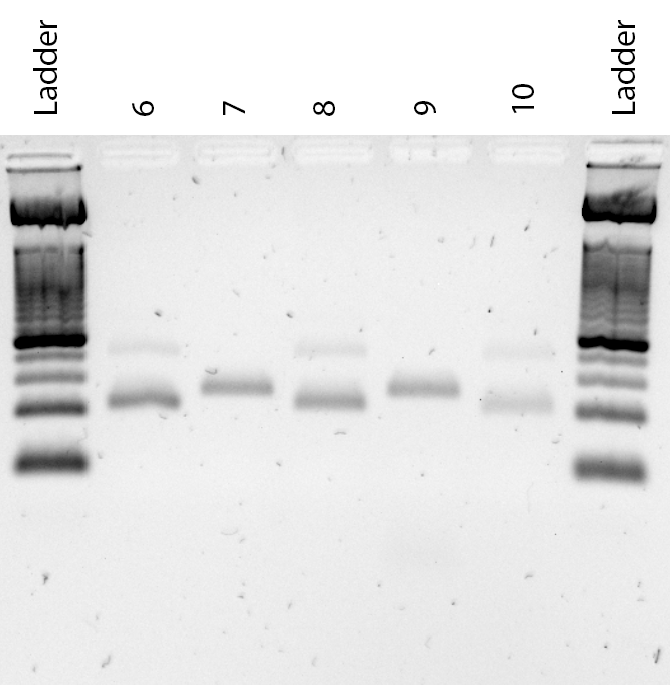
\includegraphics[width=\textwidth]{images/translator_pcr_long_1.png}
  \caption{}
  \label{translator_pcr_long_1}
\end{subfigure}
\begin{subfigure}[t]{0.47\textwidth}
  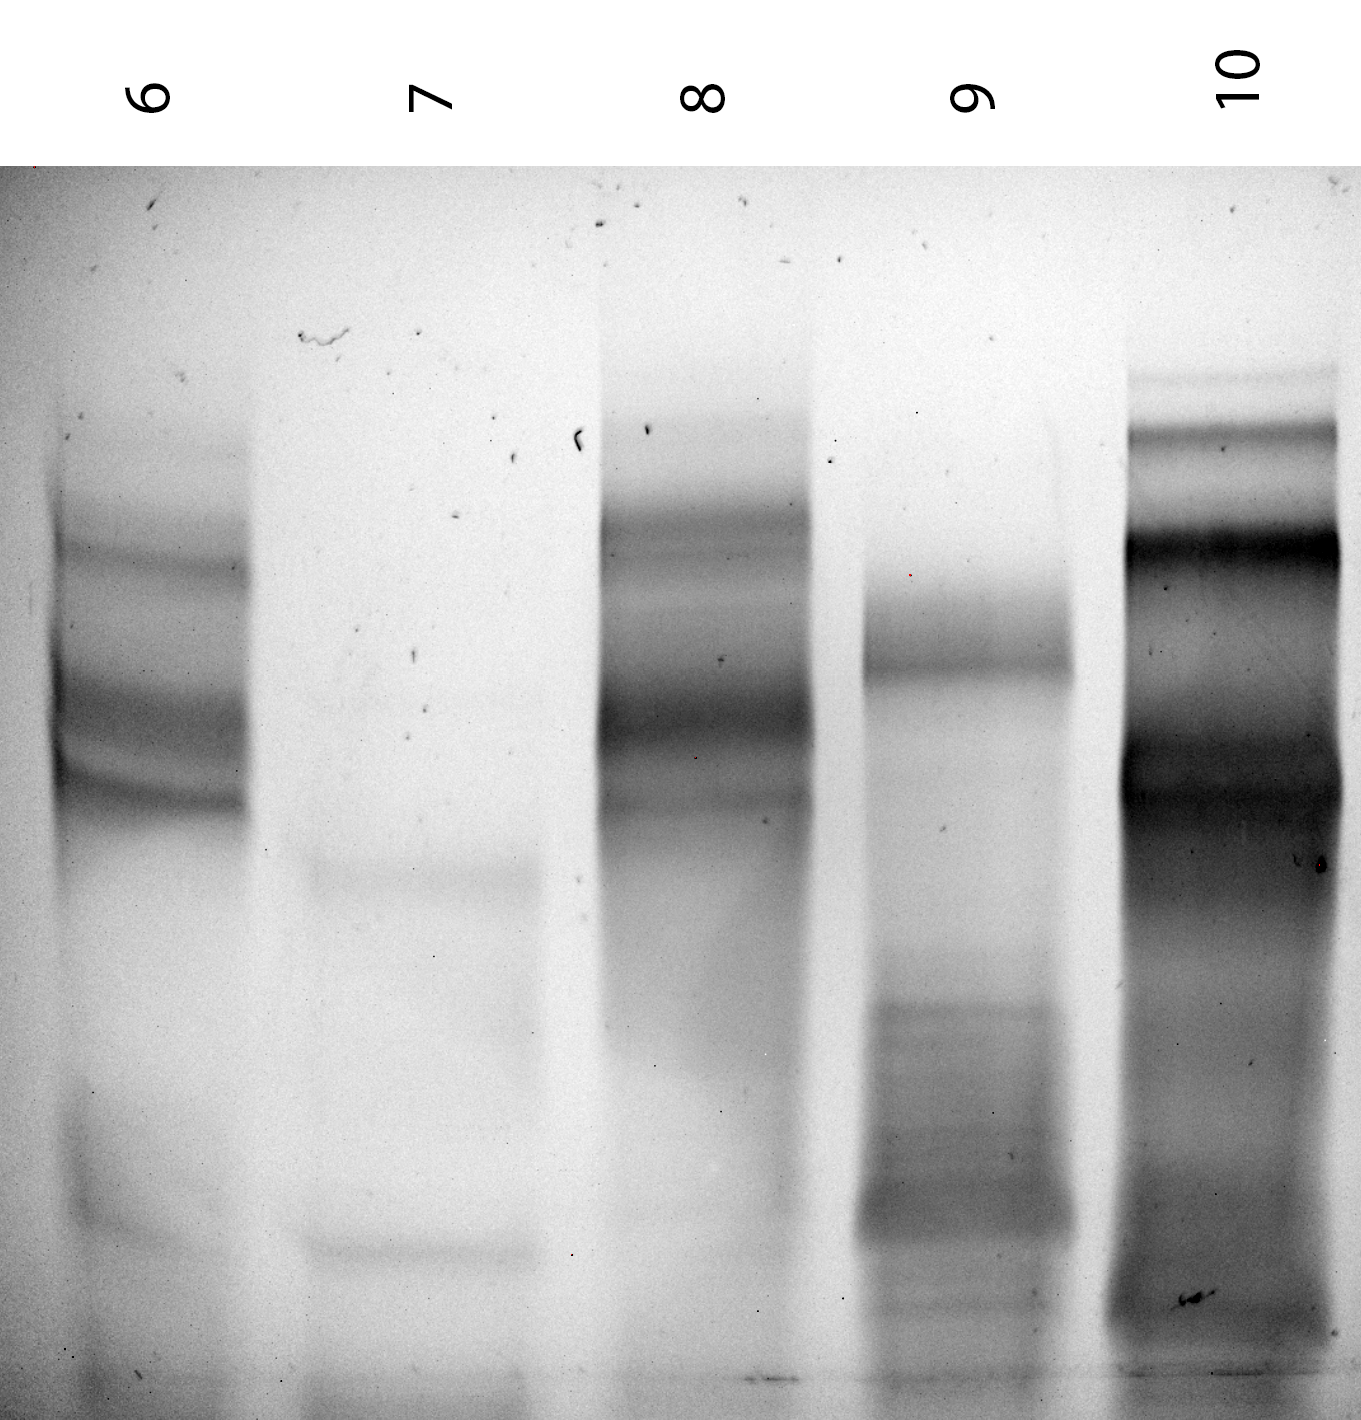
\includegraphics[width=\textwidth]{images/translator_transcription_long_ds_1.png}
  \caption{}
  \label{translator_transcription_long_ds_1}
\end{subfigure}
\caption{\subref{translator_pcr_long_1} PCR product of the long translator sequences. \subref{translator_transcription_long_ds_1} Transcription of the double-stranded long translator sequences.}
\end{figure}

The result in \fref{translator_pcr_long_1} shows the expected PCR product sizes compared with \tref{dna_strands}. Another transcription reaction was carried out on the double-stranded long translator.

\fref{translator_transcription_long_ds_1} shows strand 10 clearly, but still a lot of other products, and strand 7 has hardly been transcribed at all. The results might be explained by secondary structures of the RNA strands. If the strands form strong hairpins, the transcription can be aborted early, and produce unintended products. The RNA strands were checked in Nupack for secondary structures. Comparing the Nupack analysis in \fref{long_secondary_structures} with the gel in \fref{translator_transcription_long_ds_1}, the amount of product seems to follow the free energy of the secondary structure of the RNA. Strand 10 which was visible in UV shadowing has no secondary structure with the highest probability, and strand 7 which shows the least amount of product has the lowest free energy.

The only way to avoid this problem is to create another design which doesn't have secondary structures, but since the translator sequences are locked by the desired input and output sequences, this is not a possibility. To actually get the RNA strands, they should have been ordered from IDT, synthesized and purified. This is more expensive, and was thought to be unnecessary in the beginning of the experiment. There was not enough time left to order the RNA sequences and carry out the fluorescence measurements on the reporter, so no results was obtained from the experiment.
